\documentclass[aps,twocolumn,prd,superscriptaddress,nofootinbib,floatfix]{revtex4-2}



%%%%%%%%%%%%% Packages %%%%%%%%%%%%%

% general
%\usepackage[utf8]{inputenc}
  
% math
\usepackage{mathtools}
\usepackage{amsfonts}
\usepackage{amssymb}
\usepackage{mathrsfs}
\usepackage{bbm}
\usepackage{slashed}
\usepackage{amsmath}
\usepackage{bm}
\usepackage{bbold}


% graphics and colors
\usepackage{graphicx}
\usepackage{color}
\usepackage{colortbl}
\usepackage{array}

% floats
\usepackage{float}
\usepackage{placeins}
\usepackage{booktabs}
%\usepackage{caption}
\usepackage[caption=false]{subfig}
\captionsetup{justification=centerlast}
\usepackage{makecell}
\usepackage{tabstackengine}


% units and refs
\usepackage{xspace}
\usepackage{hyperref}
\usepackage[nameinlink]{cleveref}
\usepackage{bookmark}
\usepackage{siunitx}


% Other
\usepackage{xifthen}
\usepackage{xcolor}
\hypersetup{
	colorlinks,
	linkcolor={red!75!black},
	citecolor={blue!75!black},
	urlcolor={blue!75!black}
}

\usepackage[utf8]{inputenc}
\allowdisplaybreaks[4]


%%%%%%%%%%%%%%%%%%%%%%%%%%%%%%%%%%%%%%%%

%--- start of the macros paper%
\newcommand{\hlambda}{\hat{\lambda}}
\newcommand{\LQCD}{\Lambda_{\text{\tiny QCD}}}
\newcommand{\eb}{\epsilon_{{b}}}
\newcommand{\muq}{\mu_{\textrm{q}}}
\newcommand{\mud}{\mu_{\textrm{d}}}
\newcommand{\mub}{\mu_{{b}}}
\newcommand{\mubo}{\bar{\mu}_{{b}}}
\newcommand{\mudo}{\bar{\mu}_{\textrm{d}}}
\newcommand{\muqo}{\bar{\mu}_{\textrm{q}}}
\newcommand{\MN}{M_{\textrm{N}}}
\newcommand{\mq}{m_{\textrm{q}}}
%\renewcommand{\md}{m_{\text{d}}}
\newcommand{\Md}{M_{\text{d}}}
\newcommand{\Mq}{M_{\text{q}}}
\newcommand{\Mb}{M_{{b}}}
\newcommand{\Mqb}{M_{\text{q}/{b}}}
\newcommand{\energyq}{\varepsilon_{\text{q}}}
\newcommand{\Lag}{\mathcal{L}}
\newcommand{\ua}{\mathrm{U(1)_A}}
\newcommand{\diag}{\mathrm{diag}}
\newcommand{\MeV}{\;\text{MeV}}
\newcommand{\GeV}{\;\text{GeV}}
\newcommand{\fm}{\;\text{fm}}
\newcommand{\rmi}{\mathrm{i}}
\newcommand{\rmd}{\mathrm{d}}
\newcommand{\rme}{\mathrm{e}}
\newcommand{\Nc}{N_{\mathrm{c}}}
\newcommand{\Nf}{N_{\mathrm{f}}}
\newcommand{\Tc}{T_{\mathrm{c}}}
\newcommand{\bB}{\boldsymbol{B}}
\newcommand{\bE}{\boldsymbol{E}}
\newcommand{\bgamma}{\vec{\gamma}}
\newcommand{\tr}{\text{tr}}
\newcommand{\Tr}{{\text{Tr}}}
\newcommand{\bp}{\vec{p}}
\newcommand{\Phifund}{\Phi_{\text{\tiny{fund}}}}
\newcommand{\rhos}{\rho_{\rm \phi}}
\newcommand{\rhod}{\rho_{\rm d}}
\newcommand{\Zq}{Z_{q}}
\newcommand{\Zphi}{Z_{\phi}}
\newcommand{\Zd}{Z_{d}}
\newcommand{\ZV}{Z_{V}}
\newcommand{\Zo}{Z_{\omega}}
\newcommand{\Zb}{Z_{b}}
\newcommand{\lambdas}{\lambda_{q\phi}}
\newcommand{\lambdad}{\lambda_{qd}}
\newcommand{\lambdasd}{\lambda_{q \phi/ d}}
\newcommand{\lambdaV}{\lambda_{qV}}
\newcommand{\lambdao}{\lambda_{q\omega}}
\newcommand{\lambdab}{\lambda_{qb}}
\newcommand{\lambdabd}{\lambda_{qdb}}
\newcommand{\lambdabo}{\lambda_{b\omega}}

\newcommand{\hs}{h_{q\phi}}
\newcommand{\hd}{h_{qd}}
\newcommand{\hV}{h_{qV}}
\newcommand{\ho}{h_{q\omega}}
\newcommand{\hsd}{h_{q \phi/d}}
\newcommand{\hsb}{h_{q/b \phi}}
\newcommand{\hb}{h_{b\phi}}
\newcommand{\hbo}{h_{\omega \rm b}}
\newcommand{\hdo}{h_{\omega \rm d}}
\newcommand{\hqo}{h_{\omega \rm q}}
\newcommand{\hqdb}{h_{qdb}}
\newcommand{\hqb}{h_{qb}}
\newcommand{\dynA}{D}
\newcommand{\dynB}{D}
\newcommand{\bolda}{\boldsymbol{a}}
\newcommand{\boldabar}{\bar{\boldsymbol{a}}}
\newcommand{\feyn}[1]{
	\setbox0=\hbox{\ensuremath{#1}}
	\hbox to\wd0{\hbox to0pt{\hbox to\wd0{\hss/\hss}\hss}\box0}}

\newcommand{\nsat}{n_{b}^{\text{(sat)}}}
\newcommand{\Vb}{V_{b}}
\newcommand{\nb}{n_{b}}

%--- end of the definition of KF ---%
%%%%%%% Dirac slashes %%%%%%
\def\pslash{p\hspace{.015cm}\llap{/}\hspace{.015cm}}
\def\pa{\partial}
\def\al{\alpha}
\def\pr{\prime}
\def\dr{{D\!\llap{/}}\,}
\def\Dr{{D\llap{/}}\,}
% \def\k{k\llap{/}}
\def\ip{p\llap{/}}
\def\iq{q\llap{/}}
\def\ik{k\llap{/}}
\def\il{l\llap{/}}
\def\ir{r\llap{/}}
\def\es{\epsilon\llap{/}}
\def\A{A\!\llap{/}}
%%%%%%%%%%%% refs %%%%%%%%%%%%%%%%%%%
\def\sectionautorefname{Sec.\!}
\def\figureautorefname{Fig.\!}
\def\tableautorefname{Tab.\!}
\def\Eq#1{\Cref{#1}}
\def\Fig#1{\Cref{#1}} 
\def\Tab#1{\Cref{#1}}
%%%%%%%%%%%%% Options %%%%%%%%%%%%%
\setkeys{Gin}{width=0.48\textwidth}
\captionsetup{justification=centerlast}
\sisetup{range-units=single}

%\newcommand{\tr}{{\text{tr}}}

\newcommand*{\eg}{e.g.\@\xspace}
\newcommand*{\ie}{i.e.\@\xspace}
\newcommand*{\etc}{etc.\@\xspace}
\newcommand*{\cf}{cf.\@\xspace}


%%%%%%%%%%%%% Math commands %%%%%%%%%%%%%
% symbols
\newcommand{\sumint}{\int\hspace{-4.8mm}\sum}
\newcommand{\imag}{\text{i}}
\newcommand{\pz}{$P_z$}

\newcommand{\tinytext}[1]{\text{\tiny{#1}}}

%%%%%%%%%%%%% Graphic paths %%%%%%%%%%%%%
\graphicspath{{./figures/}}


%%%%%%%%%%%%%% for corrections %%%%%%%%%%%
\newcommand{\colsy}[1]{\textcolor{green}{#1}}

\newcommand{\gettitle}{}

% affiliations
\newcommand{\getFudanAffiliation}{\affiliation{Key Laboratory of Nuclear Physics and Ion-beam Application (MOE),
and Institute of Modern Physics, Fudan University, Shanghai 200433, China}}

\newcommand{\getNSFCFudanAffiliation}{\affiliation{Shanghai Research Center for Theoretical Nuclear Physics, NSFC and Fudan University, Shanghai 200438, China}}

\newcommand{\getDalianAffiliation}{\affiliation{School of Physics, Dalian University of Technology, Dalian, 116024, P.R. China}}

\newcommand{\getGiessenAffiliation}{\affiliation{Institut f\"ur Theoretische Physik, Justus-Liebig-Universit\"at Gie\ss en, 35392 Gie\ss en, Germany}}


\hypersetup{
	colorlinks,
	linkcolor={red!75!black},
	citecolor={blue!75!black},
	urlcolor={blue!75!black},
	%%%%%%%%%%%%%%%%%%%%%%%%%%%%%%%%%%
	pdftitle={\gettitle},
	pdfauthor={Zelle},
	pdfkeywords={effective theory} {analytic continuation}
	{correlations functions} {hadronization}
	{functional renormalisation group}
	{real time} {bound states}
	bookmarksopen=true,
	bookmarksopenlevel=2,
	bookmarksnumbered=true
}


\begin{document}

\title{Mapping the critical region along the 2nd-order phase boundary}

\author{Shi Yin}
\email{Shi.Yin@theo.physik.uni-giessen.de}
\getGiessenAffiliation

\begin{abstract} 

In this paper 

\end{abstract}
	
\maketitle


%%%%%%%%%%%%%%%%%%%%%%%%%%%%%%%%%%%%%%%%%%%%%%%%%%%%%%%%%%%%%%%%%%%%%%%%%%%%%%%%%%%%%%%%%%%%%%%%%%%%%%%%%%%%%%%%%%%%%%%%%%%%%%%%%%%%%%%%%%%%%%%%%%%%
%%%%%%%%%%%%%%%%%%%%%%%%%%%%%%%%%%%%%%%%%%%%%%%%%%%%%%%%%%%%%%%%%%%%%%%%%%%%%%%%%%%%%%%%%%%%%%%%%%%%%%%%%%%%%%%%%%%%%%%%%%%%%%%%%%%%%%%%%%%%%%%%%%%%
\section{Introduction}
This is

%%%%%%%%%%%%%%%%%%%%%%%%%%%%%%%%%%%%%%%%%%%%%%%%%%%%%%%%%%%%%%%%%%%%%%%%%%%%%%%%%%%%%%%%%%%%%%%%%%%%%%%%%%%%%%%%%%%%%%%%%%%%%%%%%%%%%%%%%%%%%%%%%%%%
%%%%%%%%%%%%%%%%%%%%%%%%%%%%%%%%%%%%%%%%%%%%%%%%%%%%%%%%%%%%%%%%%%%%%%%%%%%%%%%%%%%%%%%%%%%%%%%%%%%%%%%%%%%%%%%%%%%%%%%%%%%%%%%%%%%%%%%%%%%%%%%%%%%%
\section{quark-meson model within functional renormalization group approach}
\label{sec:QM_frg} 
As a starting point, this section introduces the quark-meson (QM) model employed in this work, along with the technical details required for the fRG approach calculations. In order to incorporate the QM model into the framework of fRG, we first formulate the scale-dependent effective action of the model
%
%%%%
\begin{align}\label{eq:action}
\Gamma_k[\phi,q,\bar{q}]&=\int_x \bigg\{
 Z_{q,k}\,\bar q\big[\gamma_\mu \partial_\mu-\gamma_0\,\hat \mu\big]q + \frac{1}{2}\,Z_{\phi,k}\,(\partial_\mu\phi)^2\nonumber\\[2ex]
&+\frac{1}{2}\,h_k\,\bar q(\tau^0 \sigma+i\gamma_5 \boldsymbol{\tau}\cdot\boldsymbol{\pi})q+U_k(\rho)-c\sigma\bigg\}\,.
\end{align}
%%%%
%
In this effective action, we have the degree of freedom of the hadrons $\phi=(\sigma,\boldsymbol{\pi})$ and the (anti-) quark ($\bar q$) $q$. The range of the Lorentz index $\mu$ is taken to be from 0 to 3. For simplicity, we consider two light-quark flavors with degenerate masses and chemical potentials, i.e., $m_q\equiv m_u=m_d$ and $\hat\mu=\mathrm{diag}(\mu,\mu)$. The interaction strength between mesons and quarks is given by the Yukawa coupling $h_k$. Then we have the tensor $\tau^0=1/\sqrt{2N_f}\mathbbm{1}_{N_f\times N_f}$ and Pauli matrices $\boldsymbol{\tau}$ with $N_f=2$ and $N_c=3$. The effective potential $U_k(\rho)$ captures the chiral phase transition at finite temperature and density together with the linear chiral symmetry breaking term $-c\sigma$. The $c$ in the linear term gives the strength of the chiral symmetry breaking which is related to the current light quark mass. When we set this strength to zero, the system reaches the chiral limit. Note that in this work our computations are carried out within both the Local Potential Approximation (LPA) and LPA'. In LPA, the scale dependence of the meson (quark) wave function renormalization $Z_{\phi/q,k}$ and the Yukawa coupling $h_k$ will not be taken into account. In LPA', we take into account the flow of meson wave function renormalization $Z_{\phi,k}$, i.e., meson anomalous dimension. In both cases we set the $Z_{q,k}=1$, because the quark wave function renormalization does not alter the critical exponents of the $O(4)$ universality class.

To solve the effective action at infrared energy scale, we have to introduce the Wetterich equation \cite{Wetterich:1992yh}
%
%%%%
\begin{align}\label{eq:wetterich_eq}
\partial_t\Gamma_k[b,q,\bar q]=\frac{1}{2}\mathrm{Tr}\bigg(G^{bb}_{k}\partial_t R^b_{k}\bigg)-\mathrm{Tr}\bigg(G^{q\bar q}_{k}\partial_t R^q_{k}\bigg)\,.
\end{align}
%%%%
%
In order to preserve the dimensional consistency of the equations, we use the renormalization group (RG) time $t=\mathrm{ln(k/\Lambda)}$. Here $\Lambda$ gives us the ultraviolet (UV) scale of our current theory, we set it to 700 MeV in this work. The index $b$ and $q$ stand for the boson and quark d.o.f. in our system, then we have $b=(\sigma, \pi)$. The trace is performed on all the intrinsic degrees of freedom, e.g., flavor, color and Lorentz space. The $G^{bb/q\bar{q}}_k$ is the propagator and the $R^{b/q}_k$ is the regulator of meson/quark, the definitions of them are given in \cref{app:flow_eq}.

We start the flow equation of the effective potential
%
%%%%
\begin{align}\label{eq:u_flow}
\partial_t U_k(\rho)=&\frac{k^4}{4\pi^2}\bigg[(N_f^2-1)l^{(b,4)}_0(m^2_{\pi,k},\eta_{\phi,k};T)\nonumber\\[2ex]
&+l^{(b,4)}_0(m^2_{\sigma,k},\eta_{\phi,k};T)\nonumber\\[2ex]
&-4N_cN_fl^{(q,4)}_0(m^2_{q,k};T,\mu)\bigg]
\end{align}
%%%%
%
The $l^{(b/q,4)}_0$ is the threshold function of a bosonic field or a quark field, the expression is also given in \cref{app:flow_eq}. In addition, they are all the functions of meson mass or quark mass. Then the dimensionless masses are defined by
%
%%%%
\begin{align}
m^2_{\pi,k}&=\frac{U_k'(\rho)}{k^2Z_{\phi,k}}\,,\\[2ex]
m^2_{\sigma,k}&=\frac{U_k'(\rho)+2\,\rho\,U_k''(\rho)}{k^2Z_{\phi,k}}\,,\\[2ex]
m^2_{q,k}&=\frac{h_k^2\rho}{2\,k^2\,Z_{q,k}}\,,
\end{align}
%%%%
%
with the $O(4)$ invariant meson field $\rho=\phi^2/2$. The meson anomalous dimension is given by $\eta_{\phi,k}=-\partial_tZ_{\phi,k}/Z_{\phi,k}$. We use the Taylor expansion method to solve the effective potential. We give the expansion form of the potential
%
%%%%
\begin{align}
U_k(\rho)=\sum^N_{n=0}\frac{\bar\lambda_{n,k}}{n!}(\bar\rho-\bar\kappa_k)^n\,.
\end{align}
%%%%
%
The expansion coefficients, meson field and the expansion point are all RG-invariant quantities. They are defined by $\bar\lambda_{n,k}=\lambda_{n,k}/Z^n_{\phi,k}$, $\bar{\rho}=\rho\,Z_{\phi,k}$ and $\bar{\kappa}_k=\kappa_k\,Z_{\phi,k}$. In this work, we expand the potential up to $N=5$, in \cite{Yin:2019ebz,Pawlowski:2014zaa} we can see that under this order sufficient convergence can already be observed. The flow equations of the Taylor coefficients can be obtained by the field derivative of \Eq{eq:u_flow}
%
%%%%
\begin{align}\label{eq:flow_coef}
&\partial_{\bar\rho}\Big(\partial_tU_k(\bar\rho)\Big)\bigg|_{\bar\rho=\bar\kappa_k}\nonumber\\[2ex]
=&(\partial_t-n\,\eta_{\phi,k})\bar{\lambda}_{n,k}-(\partial_t\bar{\kappa}_k+\eta_{\phi,k}\bar{\kappa}_k)\bar{\lambda}_{n+1,k}\,.
\end{align}
%%%%
%
The flow of the expansion point $\partial_t\bar{\kappa}_k$ is given by the gap equation of the potential
%
%%%%
\begin{align}\label{eq:gapeq}
\partial_{\bar\rho}\Big(U_k(\bar\rho)-\bar c_k\sqrt{2\bar\rho}\Big)\bigg|_{\bar\rho=\bar\kappa_k}=0\,.
\end{align}
%%%%
%
The scale dependence of the explicit chiral symmetry breaking term is only given by the meson wave function renormalization $\bar c_k=c/\sqrt{Z_{\phi,k}}$, and $\partial_t\bar c_k=\eta_{\phi,k}\bar c_k/2$. We solve the \Eq{eq:flow_coef} and \Eq{eq:gapeq} together and get the flow equation of the expansion point
%
%%%%
\begin{align}
\partial_t\bar \kappa_k=&-\frac{\bar c_k^2}{\bar\lambda^3_{1,k}+\bar c_k^2\,\bar\lambda_{2,k}}\nonumber\\
&\times\bigg\{\partial_{\bar\rho}\Big(\partial_tU_k(\bar\rho)\Big)\bigg|_{\bar\rho=\bar\kappa_k}+\eta_{\phi,k}\Big(\frac{\bar\lambda_{1,k}}{2}+\bar\kappa_k\,\bar\lambda_{2,k}\Big)\bigg\}\,.
\end{align}
%%%%
%
These equations are under the LPA' truncation. If we set $\eta_{\phi,k}=0$ and $Z_{\phi,k}=1$ at every RG-scale, we can go back to LPA truncation.

The flow equation of meson anomalous dimension is given by a momentum derivative of the meson two-point function
%
%%%%
\begin{align}\label{eq:eta_phi}
\eta_{\phi,k}=-\frac{\delta_{ij}}{3Z_{\phi,k}}\frac{\partial}{\partial(|\mathbf{p}|^2)}\frac{\delta^2\partial_t\Gamma_k}{\delta\pi_i(-p)\delta\pi_j(p)}\bigg|_{p=0}\,.
\end{align}
%%%%
%
Note that, we use the spatial component of the pion wave function renormalization in our computation. This approximation is checked in \cite{Yin:2019ebz}, at low density area this setup can ensure the $O(4)$ critical behavior very well. The numerical setup of the QM model is also given in \cref{app:flow_eq}.

For the Yukawa coupling $\bar h_k$, we do not consider the flow contribution of the quark-meson vertex. So the flow equations of it only comes from the meson anomalous dimension $\partial_t \bar h_k=\eta_{\phi,k}\bar h_k/2$.
%%%%%%%%%%%%%%%%%%%%%%%%%%%%%%%%%%%%%%%%%%%%%%%%%%%%%%%%%%%%%%%%%%%%%%%%%%%%%%%%%%%%%%%%%%%%%%%%%%%%%%%%%%%%%%%%%%%%%%%%%%%%%%%%%%%%%%%%%%%%%%%%%%%%
\section{Critical exponents at finite chemical potential}
\label{sec:exp}
The critical exponents characterize how different thermodynamic quantities diverge near the phase transition temperature. One can obtain the exponents by different methods. The most rigorous way to compute critical exponents is to solve the RG fixed-point equations, see e.g., \cite{Tetradis:1993ts,Tan:2022ksv}\colsy{[add more]}. One can also compute them with the data obtained from the effective potential at critical temperature, see e.g., \cite{Chen:2021iuo,Braun:2023qak}\colsy{[add more]}. In this work, we take the second method to reveal the behavior of the exponent at finite external parameters, e.g., temperature, chemical potential and current quark mass.

In this section, we compute the effective potential at finite temperature and density, then use the data to compute the critical behavior of the model at finite chemical potential. We mainly compute three critical exponents, i.e., $\delta$, $\beta$ and $\nu$. Moreover, we use these exponents to estimate the size of the $O(4)$ critical region along the second order phase boundary.
%%%%%%%%%%%%%%%%%%%%%%%%%%%%%%%%%%%%%%%%%%%%%%%%%%%%%%%%%%%%%%%%%%%%%%%%%%%%%%%%%%%%%%%%%%%%%%%%%%%%%%%%%%%%%%%%%%%%%%%%%%%%%%%%%%%%%%%%%%%%%%%%%%%
%
\subsection{Critical behavior}
\label{subsec:CE}
We start from the grand potential of the QM model. The potential is given by the effective potential and the chiral symmetry breaking term
%
%%%%
\begin{align}
\Omega(T,\mu,c)=U_{k_\mathrm{IR}}(\bar\rho)-c\sigma\,.
\end{align}
%%%%
%
The symmetry breaking strength $c$ is proportional to the current quark mass. So if we set $c$ to zero, the whole system is in the chiral limit. When we are in the critical region of the $O(4)$ 2nd phase transition, the potential can be consider as the singular part of the scaling function
%
%%%%
\begin{align}
f_s(t,h)\sim \Omega(\pm\epsilon_t,\epsilon_c)\,.
\end{align}
%%%%
%
If the variations in the direction of temperature and the explicit symmetry breaking term are infinitesimal, the effective potential remains within the critical region. Therefore, it can still be described by the singular equation. Here we use the reduced temperature $t=(T-T_c)/T_c$ and the external field $h$ which is related to the chiral breaking strength $c$. The order parameter of the system can be computed by the scaling function with a derivative of the external field
%
%%%%
\begin{align}
M=-\frac{\partial f_s}{\partial\,h}\equiv \sigma_0\,,
\end{align}
%%%%
%
which is the expectation value of the light quark condensate. The critical exponents $\beta$ and $\delta$ can be computed through the order parameter
%
%%%%
\begin{align}
\sigma_0(t,h=0)&\propto (-t)^\beta\,,\label{eq:beta}\\[2ex]
\sigma_0(t=0,h)&\propto h^{\frac{1}{\delta}}\label{eq:delta}\,.
\end{align}
%%%%
%
These two exponents describe the behavior of the order parameter near the critical temperature and current quark mass. In addition, there is another important critical exponent $\nu$, which characterizes the divergence of the correlation length near the critical temperature
%
%%%%
\begin{align}\label{eq:nu}
\xi\propto |t|^{-\nu}\,.
\end{align}
%%%%
%
These three exponents are computed in this work to study the critical behavior along the 2nd-order phase boundary at finite chemical potential. From the relations of exponents, we can directly obtain other exponents
%
%%%%
\begin{align}
\gamma&=\beta\,(\delta-1)\,,\\[2ex]
\gamma&=\nu\,(2-\eta)\,,\\[2ex]
\beta&=\frac{\nu}{2}\,(d-2+\eta)\,,\\[2ex]
\delta&=\frac{d+2-\eta}{d-2+\eta}\,,\\[2ex]
\nu&=\frac{\beta}{d}\,(1+\delta)\,.
\end{align}
%%%%
%
The anomalous dimension $\eta$ is also computed in the LPA' case of this work.
%%%%%%%%%%%%%%%%%%%%%%%%%%%%%%%%%%%%%%%%%%%%%%%%%%%%%%%%%%%%%%%%%%%%%%%%%%%%%%%%%%%%%%%%%%%%%%%%%%%%%%%%%%%%%%%%%%%%%%%%%%%%%%%%%%%%%%%%%%%%%%%%%%%%
\subsection{Critical temperature}
\label{subsec:CT}
%
%%%%%%%%%%%%%%%%%%%%%%%%%%%%%
\begin{figure}[t]

\includegraphics[width=0.48\textwidth]{kappa_k}
\caption{Dimensionless $O(4)$ invariant meson field as function of RG-scale k. The red and magenta dashed lines indicate the scale k at which the LPA and LPA' results deviate from the plateau.}
\label{fig:kappa_tc}
\end{figure}
%%%%%%%%%%%%%%%%%%%%%%%%%%%%%
%
We use the scaling behavior of the order parameter to find the critical temperature along the second order phase boundary. When one solving the dimensionless fRG fixed-point equations, it is common to assume that the equations are evaluated at a fixed dimensionless order parameter and to search for the corresponding fixed point of the model. Analogously, we use the dimensionless order parameter to determine whether the system is at its phase transition temperature $T_c$, corresponding to the Wilson–Fisher (WF) fixed point of a second-order transition. 

At finite temperature, we define a dimensionless effective potential by $u_k(\bar{\rho})=k^{-d}\,T^{-1}\,U_k(\bar{\rho})$.Here we have $d=3$. Then we can easily obtain the dimensionless order parameter $\bar{\rho}/(k\,T)$. So at the critical temperature, $\bar{\rho}/(k\,T)$ should be a constant and this can therefore serve as a criterion for identifying whether the model is at the critical temperature. An example is shown in \Fig{fig:kappa_tc}, where the dimensionless order parameters are plotted as functions of the RG-scale k. We observe that the order parameter vanishes in the high-scale regime and, after crossing the chiral symmetry breaking scale $k_{\chi SB}$, rapidly rises to a constant value that remains stable down to the infrared. This behavior appear in both LPA and LPA' results. In the deep infrared region, the order parameter gradually deviates from the plateau. This deviation arises from numerical limitations, as the determination of the critical temperature becomes inaccurate at very small values of k. At this level of precision, the system gradually departs from the WF fixed point. Therefore, when computing the critical exponents, we choose the value of k within the plateau region as the infrared scale of the flow equations, as indicated by the red and magenta dashed lines in \Fig{fig:kappa_tc}.

In the following, we apply this method on different chemical potential, and the corresponding critical temperature is then determined by fine-tuning.
%%%%%%%%%%%%%%%%%%%%%%%%%%%%%%%%%%%%%%%%%%%%%%%%%%%%%%%%%%%%%%%%%%%%%%%%%%%%%%%%%%%%%%%%%%%%%%%%%%%%%%%%%%%%%%%%%%%%%%%%%%%%%%%%%%%%%%%%%%%%%%%%%%%
%
\subsection{Mass direction}
\label{subsec:delta}
%
%%%%%%%%%%%%%%%%%%%%%%%%%%%%%
\begin{figure*}[t]
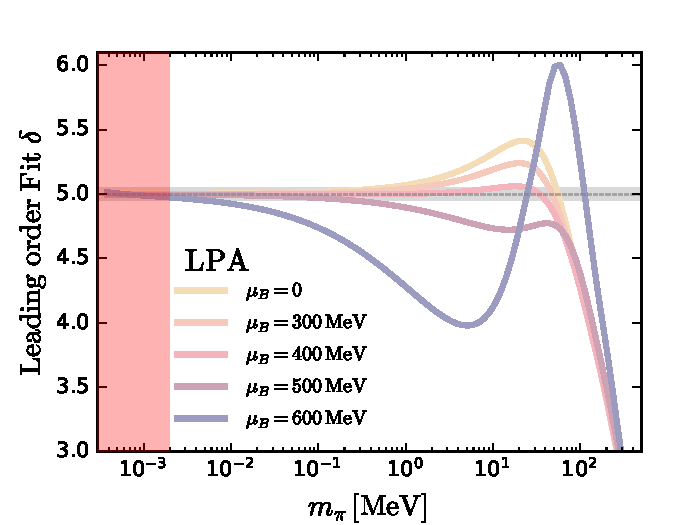
\includegraphics[width=0.48\textwidth]{delta_LO}

\includegraphics[width=0.48\textwidth]{delta_LO_LPAp}
\caption{The leading order fit of the order parameters within LPA and LPA' under different values of pion mass. The results are obtained at $\mu_B=0,\,300,\,400,\,500,\,600$ MeV for LPA and $\mu_B=0,\,300,\,400,\,500,\,530$ MeV for LPA'. The right boundary of the red band is the $k_{\mathrm{IR}}$ we choose in the computation. The gray dashed line is the value of the value of the exponent, $\delta\simeq5.0$ for LPA and $\delta\simeq4.79$ for LPA'. The gray band highlights the parameter region where the deviation of the exponent reaches $1\%$.}
\label{fig:h_scaling}
\end{figure*}
%%%%%%%%%%%%%%%%%%%%%%%%%%%%%
%
Before we start to compute the order parameter, it must be emphasized that when solving the effective potential using the Taylor expansion method, the strict chiral limit cannot be reached due to the limitations of this approach. 

We first compute the order parameter at critical temperature, i.e., $t=0$, at finite chiral symmetry breaking. We use the method introduced in \cref{subsec:CT} to determine the critical temperatures at finite chemical potential. In addition, the chiral symmetry breaking strength $c$ is proportional to the pion mass $m^2_\pi$. If we only consider the scaling part of the potential, \Eq{eq:delta} can be written as
%
%%%%
\begin{align}
\mathrm{Log}\Big(\sigma_0(t=0,m^2_\pi)\Big)=\mathrm{Log}(B_c)+\delta^{-1}\,\mathrm{Log}(m^2_\pi)+\cdots\,.
\end{align}
%%%%
%
We can see from the equation above, in the critical region, the critical exponent $1/\delta$ can be extracted by fitting the slope of $\mathrm{Log}(\sigma_0)$ versus $\mathrm{Log}(m^2_\pi)$. $\mathrm{Log}(B_c)$ denotes the amplitude factor of the data. The same method has also been employed in fRG calculations of QCD \cite{Braun:2023qak}. As the pion mass increases, the system gradually moves away from the $O(4)$ 2nd-order critical region, and the slope correspondingly deviates from the value $1/\delta$.

In \Fig{fig:h_scaling}, we demonstrate the inverse of the slope of the data as functions of pion mass at different baryon chemical potentials for both LPA and LPA'. The red band gives us the unreliable region of the data. In this region the pion mass is smaller than the infrared cutoff $k_{\mathrm{IR}}$ used in the calculation, causing the data to fall outside the range of numerical accuracy. We can see that, in the small pion mass region, the fitted slope exhibits a plateau at the value corresponding to the critical exponent $\delta$. We get the critical exponent $\delta_{\mathrm{LPA}}\simeq5.00$ and $\delta_{\mathrm{LPA}'}\simeq4.79$. For zero chemical potential, the results start to deviate from the $1\%$ vicinity of the critical exponent at the pion mass below 10 MeV, which is consistent with the QCD fits including subleading contributions \cite{Braun:2023qak}. It then exhibits a peak and rapidly decreases as the mass increases.

At high chemical potential, the data gradually change from an upward deviation to a downward deviation. In other words, the range over which the slope agrees with the critical exponent first increases and then decreases. At very high chemical potential, the LPA fit quickly deviates from the critical exponent, while the LPA' fit deviates slightly more slowly, however, the overall behavior remains similar to that of LPA.

%%%%%%%%%%%%%%%%%%%%%%%%%%%%%%%%%%%%%%%%%%%%%%%%%%%%%%%%%%%%%%%%%%%%%%%%%%%%%%%%%%%%%%%%%%%%%%%%%%%%%%%%%%%%%%%%%%%%%%%%%%%%%%%%%%%%%%%%%%%%%%%%%%%
%
\subsection{Lower temperature direction}
\label{subsec:beta}
%
%%%%%%%%%%%%%%%%%%%%%%%%%%%%%
\begin{figure*}[t]
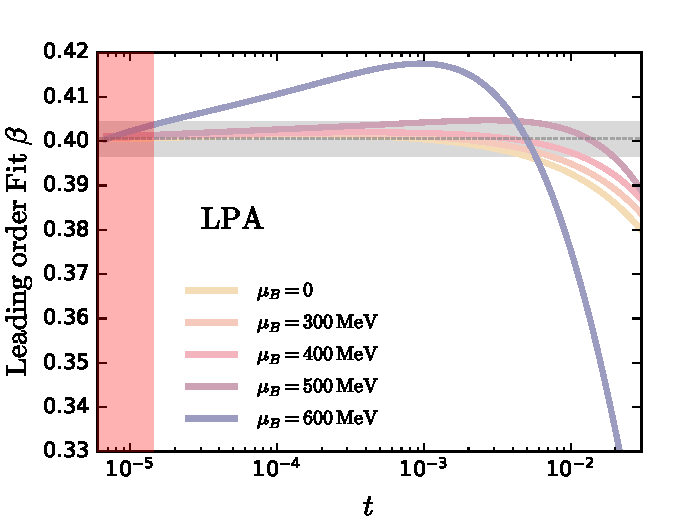
\includegraphics[width=0.48\textwidth]{beta_LO}

\includegraphics[width=0.48\textwidth]{beta_LO_LPAp}
\caption{The leading order fit of the order parameters within LPA and LPA' under different values of temperature. The results are obtained at $\mu_B=0,\,300,\,400,\,500,\,600$ MeV for LPA and $\mu_B=0,\,300,\,400,\,500,\,530$ MeV for LPA'. The gray dashed line is the value of the exponent, $\beta\simeq0.400$ for LPA and $\beta\simeq0.397$ for LPA'. The gray band highlights the parameter region where the deviation of the exponent reaches $1\%$.}
\label{fig:t_scaling}
\end{figure*}
%%%%%%%%%%%%%%%%%%%%%%%%%%%%%
%
Now we change from the mass direction to the temperature direction. Along this direction, one can start from phase transition line either to the high-temperature chiral symmetry restored phase or to the low-temperature chiral symmetry broken phase. In this subsection, we first investigate the behavior of the order parameter in the low-temperature region, i.e., the critical exponent $\beta$.

To get the order parameter as a function of temperature, we first fix the model at the  (approximate) chiral limit. In our calculations, the smallest pion mass can reach $2.7\times10^{-4}$ MeV at vacuum, which is very close to the chiral limit. In this mass, the scaling behavior of the order parameter shown in \Fig{fig:kappa_tc} can already be observed. Subsequently, we gradually lower the temperature starting from the critical temperature, i.e., the reduced temperature t is decreased from zero. From \Eq{eq:beta}, we can obtain the relation
%
%%%%
\begin{align}\label{eq:t_log}
\mathrm{Log}\Big(\sigma_0(t,h=0)\Big)=\mathrm{Log}(A)+\beta\,\mathrm{Log}(-t)+\cdots\,.
\end{align}
%%%%
%
The slope of the $\mathrm{Log}(\sigma_0)$ as function of $\mathrm{Log}(-t)$ is the exponent $\beta$. $\mathrm{Log}(A)$ is the amplitude factor along the temperature direction.

In \Fig{fig:t_scaling}, we show the results of the slope fitted by \Eq{eq:t_log}. We get the exponent $\beta_{\mathrm{LPA}}\simeq0.400$ and $\beta_{\mathrm{LPA}'}\simeq0.397$. On the temperature direction, the slope of the data is more flatten than the mass direction. For both LPA and LPA' results, the slope stays in the gray band in a wide range. In the lower-temperature region, i.e. for larger $|t|$, the LPA' results deviate from the gray band more rapidly than those of LPA. This can be attributed to the temperature dependence introduced by the anomalous dimension. As the chemical potential increases, the range over which the slope lies within the gray band first expands and then shrinks. For the results at high chemical potential, we find that the slope of the data rapidly deviates from the critical exponent within a very narrow range. This indicates that, at high chemical potential, the model quickly departs from the leading-order scaling function assumed in \Eq{eq:t_log}. To properly describe the model in this regime, additional regular corrections must be included, see, e.g., \cite{Braun:2023qak}.
%%%%%%%%%%%%%%%%%%%%%%%%%%%%%%%%%%%%%%%%%%%%%%%%%%%%%%%%%%%%%%%%%%%%%%%%%%%%%%%%%%%%%%%%%%%%%%%%%%%%%%%%%%%%%%%%%%%%%%%%%%%%%%%%%%%%%%%%%%%%%%%%%%%
%
\subsection{Higher temperature direction}
\label{subsec:nu}
%
%%%%%%%%%%%%%%%%%%%%%%%%%%%%%
\begin{figure*}[t]

\includegraphics[width=0.48\textwidth]{nu_LO}

\includegraphics[width=0.48\textwidth]{nu_LO_LPAp}
\caption{The leading order fit of the order parameters within LPA and LPA' under different values of temperature. The results are obtained at $\mu_B=0,\,300,\,400,\,500,\,600$ MeV for LPA and $\mu_B=0,\,300,\,400,\,500,\,530$ MeV for LPA'. The gray dashed line is the value of the exponent, $\nu\simeq0.804$ for LPA and $\nu\simeq0.759$ for LPA'. The gray band highlights the parameter region where the deviation of the exponent reaches $1\%$.}
\label{fig:xi_scaling}
\end{figure*}
%%%%%%%%%%%%%%%%%%%%%%%%%%%%%
%
After the lower temperature direction, we go to the other side of the phase boundary. Since in the chiral symmetry phase the order parameter is always zero, we turn to compute the critical exponent $\nu$, which is related to the correlation length of the system. From the scaling analysis, the correlation length in the $O(N)$ type model is related to the inverse mass of the $\sigma$ mode, i.e.,
%
%%%%
\begin{align}
\xi\propto\frac{1}{m_\sigma}\,.
\end{align}
%%%%
%
Because in the high temperature region the chiral symmetry is restored, the sigma mass and pion mass are the same. So here we also have $\xi\propto1/m_\pi$. So from \Eq{eq:nu} we can have the scaling relation of the data
%
%%%%
\begin{align}
\mathrm{Log}\Big(m_\sigma(t,h=0)\Big)=-\mathrm{Log}(C)-\nu\,\mathrm{Log}(t)+\cdots\,.
\end{align}
%%%%
%
The factor $\mathrm{Log}(C)$ is the amplitude of the data and $\nu$ is the critical exponent. 

In \Fig{fig:xi_scaling}, we show the slope of $\mathrm{Log}(m_\sigma)$ as function of $\mathrm{Log}(t)$ at finite reduced temperature. At low chemical potential, the behavior of the slope is similar to that of the order parameter slope in \Fig{fig:t_scaling}: it remains within a $\pm1\%$ window around the critical exponent $\nu_{\mathrm{LPA}}\simeq0.804$ and $\nu_{\mathrm{LPA}'}\simeq0.759$ over a wide range when moving away from the phase transition temperature. At finite chemical potential, the slope gradually changes from an upward deviation to a downward deviation from the critical exponent. At an intermediate value of the chemical potential, the entire curve lies within the critical exponent error window. For LPA it is around $\mu_B\sim400$ MeV, and for LPA' is around $\mu_B\sim420$ MeV.
%%%%%%%%%%%%%%%%%%%%%%%%%%%%%%%%%%%%%%%%%%%%%%%%%%%
%%%%%%%%%%%%%%%%%%%%%%%%%%%%%%%%%%%%%%%%%%%%%%%%%%%
\section{Conclusions}
\label{sec:conclusion}

%%%%%%%%%%%%%%%%%%%%%%%%%%%%%%%%%%%%%%%%%%%%
\section*{Acknowledgements}

We thank .... This work is supported by 

%%%%%%%%%%%%%%%%%%%%%%%%%%%%%%%%%%%%%%%%%%%%%%%%%%%%%%%%%%%%
%%%%%%%%%%%%%%%%%%%%%%%%%%%%%%%%%%%%%%%%%%%%%%%%%%%%%%%%%%%%
\appendix 
%%%%%%%%%%%%%%%%%%%%%%%%%%%%%%%%%%%%
\section{flow equations}
\label{app:flow_eq}

In the computation of the flow equations, we use the 3d-flat Litim regulator functions \cite{Litim:2000ci} for both boson and fermion
%
%%%%
\begin{align}
R^b_k(\mathbf{q})&=Z_{\phi,k}\,\mathbf{q}^2\,r_b(\mathbf{q}^2/k^2)\,,\\[2ex]
R^q_k(\mathbf{q})&=Z_{q,k}\,i\,\bm{\slashed{q}}\,r_f(\mathbf{q}^2/k^2)\,.
\end{align}
%%%%
%
The shape function is defined by the Heaviside theta function
%
%%%%
\begin{align}
r_b(x)&=\bigg(\frac{1}{x}-1\bigg)\Theta(1-x)\,,\\[2ex]
r_f(x)&=\bigg(\frac{1}{\sqrt x}-1\bigg)\Theta(1-x)\,.
\end{align}
%%%%
%
Then the dimensionless propagators of boson and fermion as follows
%
%%%%
\begin{align}
G_b(q,m^2_b)&=\frac{1}{\tilde q_0^2+1+m^2_{b,k}}\,,\\[2ex]
G_q(q,m^2_q;\tilde \mu)&=\frac{1}{(\tilde q_0+i\tilde\mu)^2+1+m^2_{q,k}}\,.
\end{align}
%%%%
%
The $\tilde\mu=\mu/k$ and $\tilde q_0=q_0/k$ are the dimensionless quark chemical potential and Matsubara frequency.

The threshold functions which are used in the flow equation of effective potential is
%
%%%%
\begin{align}
l_0^{(b,d)}(m^2_{b,k},\eta_{\phi,k};T)&=\frac{2}{d-1}\bigg(1-\frac{\eta_{\phi,k}}{d+1}\bigg)\mathcal{B}_{(1)}(m^2_{b,k};T)\,,\\[2ex]
l_0^{(q,d)}(m^2_{q,k},\eta_{q,k};T,\mu)&=\frac{2}{d-1}\bigg(1-\frac{\eta_{q,k}}{d}\bigg)\mathcal{F}_{(1)}(m^2_{q,k};T,\mu)\,.
\end{align}
%%%%
%
In the computation we use $d=4$ and $\eta_{q,k}=0$. The definition of the boson and fermion threshold functions $\mathcal{B}_{(n)}$ and $\mathcal{F}_{(n)}$ are the Matsubara summation of the propagators
%
%%%%
\begin{align}
\mathcal{B}_{n}(m^2_{b,k},T)&=\frac{T}{k}\sum_{n_0}\Big(G_b(q,m^2_{b,k})\Big)^n\,,\\[2ex]
\mathcal{F}_{n}(m^2_{q,k},T,\mu)&=\frac{T}{k}\sum_{n_0}\Big(G_q(q,m^2_{q,k})\Big)^n\,.
\end{align}
%%%%
%
The lowest order of the functions are given by
%
%%%%
\begin{align}
\mathcal{B}_{(1)}(m^2_{b,k},T)&=\frac{1}{\sqrt{1+m^2_{b,k}}}\bigg(\frac{1}{2}+n_b(m^2_{b,k},T)\bigg)\,,\\[2ex]
\mathcal{F}_{(1)}(m^2_{q,k};T,\mu)&=\frac{1}{2\sqrt{1+m^2_{q,k}}}\\
\times\bigg(1-&n_q(m^2_{q,k};T,\mu)-n_q(m^2_{q,k};T,-\mu)\bigg)\,.
\end{align}
%%%%
%
The definitions of the boson and fermion distribution functions are
%
%%%%
\begin{align}
n_b(m^2_{b,k};T)&=\frac{1}{\mathrm{exp}\Big[\frac{k\sqrt{1+m^2_{b,k}}}{T}\Big]-1}\,,\\[2ex]
n_q(m^2_{q,k};T,\pm\mu)&=\frac{1}{\mathrm{exp}\Big[\frac{k\sqrt{1+m^2_{q,k}}\mp\mu}{T}\Big]+1}\,.
\end{align}
%%%%
%

The flow equation of the meson anomalous dimension can be obtained by \Eq{eq:eta_phi} as follows
%
%%%%
\begin{align}
\eta_{\phi,k}&=\frac{1}{6\pi^2}\bigg\{\frac{4}{k^2}\bar{\kappa}_k\,\big(\bar{U}_k''(\bar{\kappa}_k)\big)^2\mathcal{BB}_{(2,2)}(m^2_{\pi,k},m^2_{\sigma,k};T)\nonumber\\[2ex]
&+N_c\,\bar{h}_k^2\Big[-3\,\mathcal{F}_{(2)}(m^2_{q,k};T,\mu)+8\,\mathcal{F}_{(3)}(m^2_{q,k};T,\mu)\Big]
\bigg\}\,.
\end{align}
%%%%
%
The double meson threshold function is given by
%
%%%%
\begin{align}
&\mathcal{BB}_{(n_1,n_2)}(m_{b_1}^2,m_{b_2}^2;T)\nonumber\\[2ex]
=&\frac{T}{k}\sum_{n_0}\bigg(G_b(q,m^2_{b_1,k})\bigg)^{n_1}\bigg(G_b(q,m^2_{b_2,k})\bigg)^{n_2}\,.
\end{align}
%%%%
%
The lowest order of the function is
%
%%%%
\begin{align}
&\mathcal{BB}_{(1,1)}(m^2_{b_1},m^2_{b_2};T)\nonumber\\[2ex]
=&-\bigg\{\bigg(\frac{1}{2}+n_b(m^2_{b_1,k};T)\bigg)\,\frac{1}{\sqrt{1+m^2_{b_1,k}}(m^2_{b_1}-m^2_{b_2})}\nonumber\\[2ex]
&\,\,\,\,\,\,\,+\bigg(\frac{1}{2}+n_b(m^2_{b_2,k};T)\bigg)\,\frac{1}{\sqrt{1+m^2_{b_2,k}}(m^2_{b_2}-m^2_{b_1})}
\bigg\}\,.
\end{align}
%%%%
%
The higher order of the threshold functions can be obtained by the derivative of the first order of the function with respect to the masses. For example
%
%%%%
\begin{align}
&\mathcal{BB}_{(n_1+1,n_2)}(m^2_{b_1,k},m^2_{b_2,k};T)\nonumber\\[2ex]
=&-\frac{1}{n_1}\frac{\partial}{\partial\,m^2_{b_1,k}}\mathcal{BB}_{(n_1,n_2)}(m^2_{b_1,k},m^2_{b_2,k};T)\,.
\end{align}
%%%%
%
%%%%%%%%%%%%%%%%%%%%%%%%%%%%%%%%%%%%
\section{Numerical setup}
\label{app:numerical}
Here we introduce the numerical setup of the fRG flow equations. First, we set the UV cutoff scale of the theory to $\Lambda=500$ MeV. Because our model is a low energy effective theory, so the choice of a small cutoff scale is reasonable. This small scale is also used in, e.g., \cite{Chen:2021iuo}. The behavior of the critical exponents at finite chemical potential does not depend on the value of the cutoff scale. We will show this later.

For the effective potential, we have the form at UV scale as follow
%
%%%%
\begin{align}
U_\Lambda(\rho)=\frac{\lambda_\Lambda}{2}\rho^2+\nu_\Lambda\,\rho\,.
\end{align}
%%%%
%
For both LPA and LPA', we give the parameter setup in \Tab{tab:param-set}.
%
%%%%%%%%%%%%%%%%%%%%%%%%%%%%%
\begin{table}[h]
  \begin{center}
 \begin{tabular}{ccc}
    \hline\hline & & \\[-2ex]   
    \hspace{0.5cm} $\Lambda=500$ $[\mathrm{MeV}]$& LPA & \hspace{0.5cm} LPA' \\[1ex]
    \hline & &  \\[-2ex]
   $\lambda_{\Lambda}$   & 5.7  & 5.7 \\[1ex]
   $\nu_{\Lambda}$ $[\mathrm{GeV}^2]$  & 0.290 & 0.384   \\[1ex]
   \hspace{0.5cm}$c_\sigma$ $[\times10^{-3}\mathrm{GeV}^3]$\hspace{0.5cm}   & 1.7 & 2.1  \\[1ex]
   $\bar h_\Lambda$  & 6.50 & 7.81  \\[1ex]
   \hspace{0.5cm} $m_\pi$ $[\mathrm{MeV}]$ \hspace{0.5cm} & 135.62 & 137.47 \\[1ex]
   \hspace{0.5cm} $m_\sigma$ $[\mathrm{MeV}]$ \hspace{0.5cm} & 408.36 & 387.95 \\[1ex]
   \hspace{0.5cm} $m_q$ $[\mathrm{MeV}]$ \hspace{0.5cm} & 300.41 & 300.47 \\[1ex]
   \hspace{0.5cm} $\sigma_0$ $[\mathrm{MeV}]$ \hspace{0.5cm} & 92.43 & 92.47 \\[1ex]
    \hline\hline
  \end{tabular}
  \caption{Parameters setup of the QM model with both LPA and LPA'.}
  \label{tab:param-set}
  \end{center}\vspace{-0.5cm}
\end{table}
%%%%%%%%%%%%%%%%%%%%%%%%%%%%%
%
In the LPA' approximation, the initial condition of the meson wave function renormalization is $Z_{\phi,\Lambda}=1$.


\vfill 

\bibliography{ref-lib}% 

\end{document} 